\subsection{Данные для обучения и извлечение эмбеддингов}

Здесь мы практически полностью повторяем описанный в~\cite{isrpaper} подход.
Единственным (но очень существенным) отличием является использованная размерность
эмбеддингов. Перед тем как перейти к обсуждению этого момента, расскажем про
исходные данные.

Итак, для обучения и тестирования моделей мы использовали датасет
TIMIT\cite{timit}. Он составлен из аудиозаписей речи 630~дикторов, говорящих на
8~основных диалектах американского английского языка. Эти дикторы поделены на
обучающую (\texttt{train}) и тестовую (\texttt{test}) выборки, в первую входят
468~дикторов, во вторую --- 162. Для обучения нейросетевых моделей мы также
создавали валидационную выборку, в которую выделялись 20\% дикторов из обучающей.

Каждый из дикторов произносит 10~фонетически насыщенных предложений. При этом 2
из 10 предложений являются общими для всех дикторов
\footnote{Общие предложения:\\
          \textit{She had your dark suit in greasy wash water all year.}\\
          \textit{Don't ask me to carry an oily rag like that.}}
, остальные 8 уникальны для каждого диктора. Такое разделение позволяет без
особых затруднений подготовить данные, необходимые для описанной
в~\ref{ssec:isr} игры:
\begin{itemize}
    \item 2~общих предложения можно использовать для получения аудиозаписей
    слов.  Для этого разделим аудиозаписи этих предложений по временным
    отметкам, предоставленным создателями датасета. В результате получим 20
    аудиозаписей слов\footnote{Аналогично~\cite{isrpaper} мы не используем слово
    \textit{an}.} для каждого диктора.
    \item 8~уникальных для каждого диктора предложений можно использовать для
    получения голосовых подписей --- эмбеддингов дикторов --- просто при помощи
    усреднения эмбеддингов аудиозаписей этих предложений.
\end{itemize}

В качестве векторов признаков использовались эмбеддинги
\xvector{}~\cite{xvectorspaper}. Весь процесс преобразования аудиозаписей в
векторы признаков осуществлялся с помощью библиотеки Kaldi~\cite{kaldi}. На
первом этапе рассчитывалиcь мел-частотные кепстральные коэффициенты\footnote{
Параметры аналогичны использованным в~\cite{isrpaper} и определяются
требованиями предобученной модели.} и производилось детектирование голосовой
активности (\textit{aнгл.} VAD --- voice activity detection). Полученные векторы
признаков поступали на вход предобученной нейронной сети~\cite{sre16model}. В
качестве эмбеддингов использовались данные со второго 512-мерного слоя.

Здесь, как уже было сказано ранее, мы отступаем от оригинальной
работы~\cite{isrpaper}, где использовались 128-мерные эмбеддинги. На это есть
две причины. Во-первых, из приведенных в~\cite{isrpaper} комментариев
неочевидно\footnote{
    Цитата: \textit{We then process the MFCCs features through a pretrained
    X-Vector network to obtain a high quality voice embedding of fixed dimension
    128, where the X-Vector network is trained on augmented Switchboard, Mixer~6
    and NIST SREs}.
}, как производилось понижение размерности.
Во-вторых, мотивация такого преобразования тоже неочевидна. Уже первые проведенные
нами эксперименты показали, что при использовании 512-мерных эмбеддингов точность
идентификации оказывается существенно выше приведенных в~\cite{isrpaper} значений.

\subsection{Обучение \guesser{}}

Первой обучается нейронная сеть \guesser{}, выполняющая выбор из $K$ дикторов
при помощи $T$ аудиозаписей произнесенных слов. Как уже было сказано ранее,
эта нейросеть тренируется в режиме обучения с учителем, дикторы и произносимые
слова выбираются случайно, в качестве функции используется кросс-энтропия.
Процесс вычисления значения функции потерь для одной игры можно записать
следующим образом:
\begin{lstlisting}[caption={Рассчёт функции потерь \guesser{}}]
speaker_ids = speakers.sample(size=K)
G = voice_prints.get(speaker_ids)
target = randrange(0, K)
word_inds = randrange(0, V, size=T)
X = word_vocab.get(speaker=speaker_ids[target],
                   words=word_inds)
probabilities = guesser.forward(G, X)
loss = cross_entropy(probabilities, target)
\end{lstlisting}

Из-за увеличения относительно \citeisr{} размерности эмбеддингов пропорционально
увеличились и размерности слоёв \guesser{}. Из-за этого нам пришлось изменить
гиперпараметры, в частности мы сильно уменьшили темп обучения
(\textit{learning rate}).

Как и в оригинальной статье, для сравнения моделей будем строить графики
\textit{word} и \textit{guest sweep}. Т.~е. будем обучать модель в режиме с $K =
5$ дикторами и $T = 3$ запрашиваемыми словами, а затем будем тестировать её в
режимах с отличным числом дикторов или слов. Здесь и далее, если это не оговорено
отдельно, для расчёта точности проводятся $20000$ игр среди дикторов из тестовой
выборки, эксперименты повторяются по 5~раз c различным \texttt{seed} генератора
случайных чисел.

\begin{figure}[htb]
    \centering
    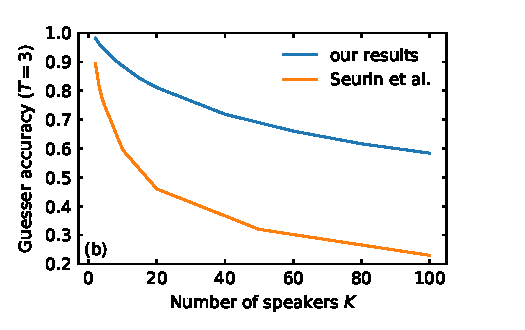
\includegraphics[scale=1.0]{../plots/guest_sweep.pdf}
    \caption{Зависимость точности \guesser{} обученного нами и авторами
    \citeisr{} от числа дикторов $K$. Модели обучены в режиме $K = 5$, $T = 3$.}
\end{figure}

\begin{figure}[htb]
    \centering
    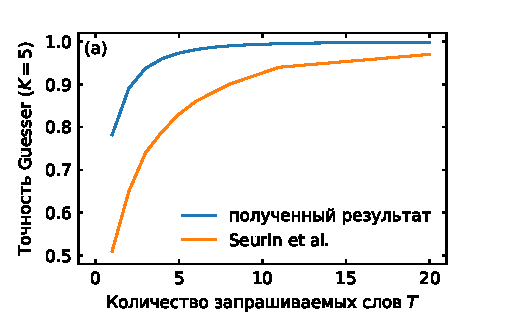
\includegraphics[scale=1.0]{../plots/word_sweep.pdf}
    \caption{Зависимость точности \guesser{} обученного нами и авторами
    \citeisr{} от числа запрошенных слов $T$. Модели обучены в режиме $K = 5$,
    $T = 3$.}
\end{figure}

По приведенным на графиках результатам видно, что увеличение размерности
эмбеддингов существенно улучшает точность идентификации, разница особо
велика в режимах с большим числом дикторов $K$.

\subsection{Обучение \enquirer{}}

Для обучения \enquirer{} --- модели выбора слов --- уже нужна обученная модель
\guesser{}. На этом этапе уже используется обучение с подкреплением, псевдокод
для 1~игры приведён ниже.
\begin{lstlisting}[caption={Интерактивная игра для обучения \enquirer{}}]
speaker_ids = speakers.sample(size=K)
G = voice_prints.get(speaker_ids)
target = randrange(0, K)

g_hat = G.mean(dim=0)
x_i = start_tensor
X = []
for i in range(T):
    probs = enquirer.forward(g_hat, x_i)
    if training:
        word_inds = multinomial(probs).sample()
    else:
        probs[previous_actions] = 0.0
        word_ind = argmax(probs)
    x_i = word_vocab.get(speaker=speaker_ids[target],
                         word=word_ind)
    X.append(x_i)

prediction = guesser.predict(G, X)
reward = 1 if prediction == target else 0
\end{lstlisting}

Как видно из приведенного псевдокода, награда выдается в том случае, когда
\guesser{} правильно угадывает диктора. Для обучения мы использовали алгоритм
PPO~\cite{schulman2017proximal} --- здесь мы снова повторяем подход
авторов~\citeisr{}. В целом выбор метода выглядит разумным --- PPO
зарекомендовал себя как простой и универсальный алгоритм, позволяющий достигать
хороших результатов. Однако некоторые особенности нашей задачи --- дискретное
пространство действий, малая длительность эпизодов --- выглядят лучше подходящими
для off-policy алгоритмов. К сожалению, у нас не нашлось времени, чтобы проверить
эту гипотезу.

\begin{figure}[htb]
    \centering
    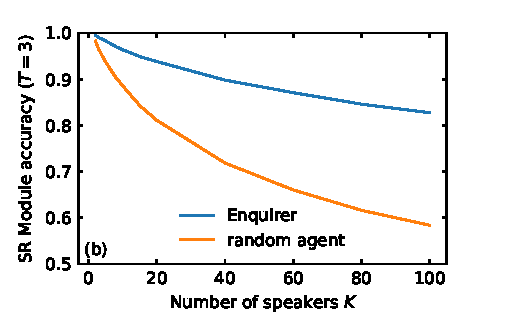
\includegraphics[scale=1.0]{../plots/guest_sweep_enq.pdf}
    \caption{Зависимость точности SR-систем с различными методами выбора слов
    --- нейросетевым агентов (\enquirer{}) и случайным (random agent) --- от
    числа дикторов $K$. Модели обучены в режиме $K = 5$, $T = 3$.}
\end{figure}

\begin{figure}[htb]
    \centering
    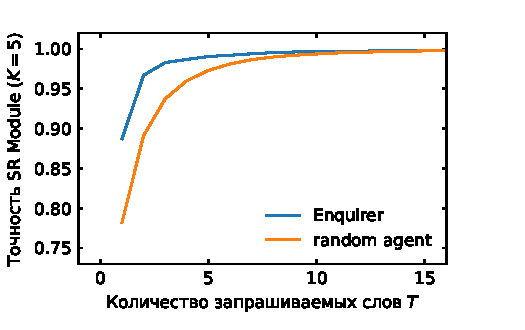
\includegraphics[scale=1.0]{../plots/word_sweep_enq.pdf}
    \caption{Зависимость точности SR-систем с различными методами выбора слов
    --- нейросетевым агентов (\enquirer{}) и случайным (random agent) --- от
    числа запрашиваемых слов $T$. Модели обучены в режиме $K = 5$, $T = 3$.}
\end{figure}

Приведенные результаты свидетельствуют о том, что \enquirer{} действительно
успешно обучается --- точность оказываются заметно выше, чем с случае
случайного выбора слов. Как и в случае повышения размерности эмбеддингов,
особенно большое различие наблюдается в режимах с большим числом дикторов.

\subsection{Эвристическая модель выбора слов}

Очевидно, что агент, выбирающий запрашиваемые слова случайным образом, не
является тяжелым противником для нейросетевого агента. Для более трезвой
оценки возможностей последнего, логично сравнивать его с каким-то более сложным
алгоритмом.

Здесь мы снова немного отходим от оригинальной статьи. И опять основной
причиной является тот факт, что в \citeisr{} отсутствует точное описание
использованного в качестве бейзлайна эвристического алгоритма выбора слов.
Из приведенных в работе слов\footnote{
    Цитата: \textit{We curated a list of the most discriminant
    words (words that increase globally the recognition scores)
    and sample among those instead of the whole list.}
}
общий подход понятен --- сэмплирование производится не из всех $20$ слов, а
из тех, которые в среднем показывают самую высокую точность. При этом остаются
непонятными следующие детали:
\begin{enumerate}
    \item Из скольки слов производится сэмплирование, и меняется ли это число
    в зависимости от числа запрашиваемых слов $T$?
    \item Производится ли сэмплирование равномерно, или вероятность выбрать
    слово пропорциональна достигаемой при выборе этого слова средней точности?
\end{enumerate}

Именно такие вопросы возникли у нас при создании эвристического агента. Первым
же этапом стала оценка слов --- расчёт средней точности, которая достигается
случайным агентом в тех играх, когда он выбрал то или иное слово. Для этого мы
протестировали \guesser{} в $100000$ эпизодов с $K = 5$, и $T = 3$, а также
случайным выбором слов без повторений. Мы рассчитывали точность для каждого слова,
учитывая только те эпизоды, в которых это слово было выбрано. Фактически мы оценивали
условную вероятность связки \guesser{}--случайный агент правильно выбрать диктора
при условии, что одно слово уже было выбрано. \hl{ссылка на рисунок}

\begin{figure}[htb]
    \centering
    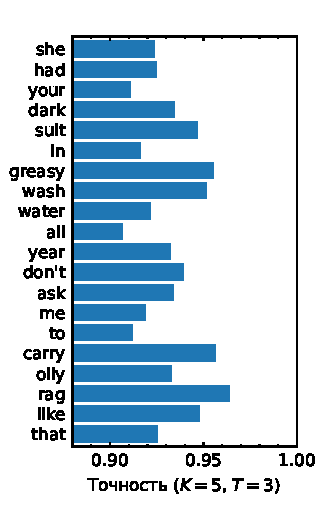
\includegraphics[scale=1.0]{../plots/word_scores.pdf}
    \caption{Средняя точность \guesser{} на валидационной выборке в тех
    эпизодах, когда соответствующее слово было выбрано (остальные выбирались
    случайно).}
\end{figure}

После этого мы стали тестировать различные модификации эвристического агента.
Как следует из сформулированных выше вопросов, эти агенты отличались числом
использованных слов и методом сэмплирования. Эксперименты показали, что
наилучшие результаты достигаются при использовании ``детерминированного'' агента,
всегда выбирающего одни и те же слова с наибольшей средней точностью.
В таком случае говорить о каком-либо сэмплировании неуместно, поэтому такой
агент, по всей видимости, отличается от использованного в оригинальной статье.

\begin{figure}[htb]
    \centering
    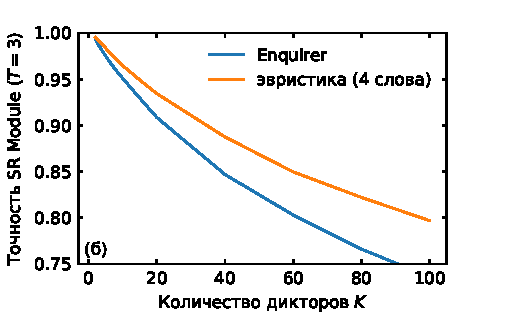
\includegraphics[scale=1.0]{../plots/guest_sweep_heuristic.pdf}
    \caption{Зависимость точности SR-систем с различными методами выбора слов
    --- нейросетевым и эвристическим агентами --- от
    числа дикторов $K$. Модели обучены в режиме $K = 5$, $T = 3$.}
\end{figure}

\begin{figure}[htb]
    \centering
    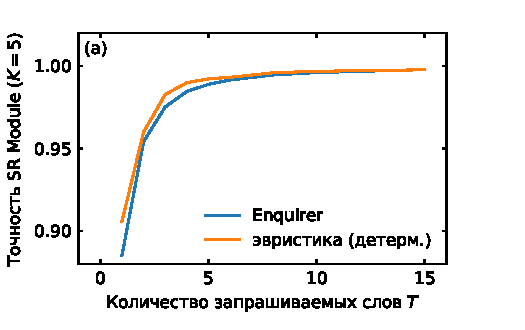
\includegraphics[scale=1.0]{../plots/word_sweep_heuristic.pdf}
    \caption{Зависимость точности SR-систем с различными методами выбора слов
    --- нейросетевым и эвристическим агентами --- от
    числа запрашиваемых слов $T$. Модели обучены в режиме $K = 5$, $T = 3$.}
\end{figure}

В данном случае преимущество \enquirer{} проявляется только в режимах с большим
числом дикторов. В стандартном режиме с $K = 5$ дикторами и $T = 3$, в отличие
от~\citeisr{}, мы не наблюдаем сколько-нибудь существенной разницы между двумя
агентами.

В таком случае возникает резонный вопрос --- не сходится ли \enquirer{}
к такой же политике, что использует эвристический агент? Ответ на этот вопрос ---
отрицательный, в целом \enquirer{} выбирает из 5 слов (ещё 2 используются редко),
в то время как эвристический агент всегда использует 3 тех же слова. Из этого
можно предположить, что \enquirer{} обучен недостаточно хорошо, возможно, другие
гиперпараметры или алгоритм обучения позволили бы улучшить результаты.

\subsection{Обучение в других режимах}

Другой логичный вопрос, возникающий при обсуждении графиков \textit{word} и
\text{guest sweep} --- является ли стандартный режим ($K = 5$ дикторов и
$T = 3$ запрашиваемых слова) оптимальным для обучения моделей? Не будут ли
результаты лучше, если мы будем обучать и тестировать модели в одном и том же
режиме? Мы также провели ряд экспериментов и пришли к следующим выводам:
\begin{itemize}
    \item Общее правило --- более тяжелые режимы позволяют улучшить точность.
    В первую очередь это касается увеличения числа дикторов, ситуация с
    уменьшением числа слов менее однозначная.
    \item Основные улучшения наблюдаются в работе \guesser{}, в то же время
    \enquirer{} оказывается нечувствительным к режиму обучения.
    \item Обучение при $T = 1$ является специфической задачей. Во-первых,
    только в этом режиме обученная модель показывает хорошие (лучше чем другие)
    результаты только в этом же режиме тестирования. Во-вторых, \enquirer{}
    в среднем показывает плохие результаты в данном режиме, часто уступая
    максимально простой политике, всегда выбирающей одно и то же слово.
\end{itemize}